\section{FuzzBench Reports}
\label{sec:report}

FuzzBench starts reporting after building the project in a local experiment. Building AFL and Waffle on a benchmark such as \textit{libpng-1.2.56} took 30 minutes on the local computer, and FuzzBench doesn't generate any reports automatically.

We tested Waffle in 6-hours experiments. Unfortunately, the local computer could not run an experiment with more than \textbf{two Fuzzers} and \textbf{one benchmark}. A more robust computer and using cloud platforms can enhance the performance of FuzzBench. Each experiment contains \textbf{3} trials for each fuzzer.

Our experiments are:

\begin{enumerate}
    \item Waffle vs AFL on libpng-1.2.56
    \item Waffle vs AFL on sqlite3\_ossfuzz
    \item Waffle vs AFL on openthread-2019-12-23
    \item Waffle vs AFL on php\_php-fuzz-execute
    \item Waffle vs AFL on curl\_curl\_fuzzer\_http
    \item Waffle vs LibFuzzer on libpng-1.2.56
    \item Waffle vs LibFuzzer on php\_php-fuzz-execute
    \item Waffle vs LibFuzzer on openthread-2019-12-23 (2x)
\end{enumerate}

We evaluate the results according to the generated reports. The graphs [Figures \ref{fig:report-log}, \ref{fig:report-box}, \ref{fig:report-unq}] illustrate the covered regions of the code in each experiment, the pairwise unique coverage, and the growth of the coverage over time. None of the experiments could find any vulnerabilities within 6 hours time limit.

\begin{table}
    \begin{adjustbox}{angle=90}
        {\setlength{\extrarowheight}{2ex}%
        \begin{tabular}{|l|c|c|c|c|c|c|} 
        \hline
        \textbf{Benchmark}                & \textbf{Fuzzer}    & \begin{tabular}[c]{@{}c@{}}\textbf{Waffle}\\ \textbf{Mean Coverage}\end{tabular} & \begin{tabular}[c]{@{}c@{}}\textbf{Fuzzer}\\ \textbf{Mean Coverage}\end{tabular} & \begin{tabular}[c]{@{}c@{}}\textbf{Waffle}\\ \textbf{STD}\end{tabular} & \begin{tabular}[c]{@{}c@{}}\textbf{Fuzzer}\\ \textbf{STD}\end{tabular} & \begin{tabular}[c]{@{}c@{}}\textbf{Unique}\\ \textbf{(Waffle/Fuzzer)}\end{tabular}  \\[2ex] 
        \hline
        libpng-1.2.56            & AFL       & 1509                                                           & 1510                                                           & 0.57                                                 & 0.57                                                 & 0/1                                                               \\[2ex] 
        \hline
        libpng-1.2.56            & LibFuzzer & 1509                                                           & 1951                                                           & 0.57                                                 & 6.65                                                 & 0/425                                                             \\[2ex]
        \hline
        php\_php-fuzz-execute    & AFL       & 147945                                                         & 169447                                                         & 5451.77                                              & 2069.34                                              & 1270/18902                                                        \\[2ex]
        \hline
        php\_php-fuzz-execute    & LibFuzzer & 145816                                                         & 138666                                                         & 2580.20                                              & 234.08                                               & 10179/335                                                         \\[2ex] 
        \hline
        openthread-2019-12-23    & AFL       & 5226                                                           & 5216                                                           & 12.58                                                & 24.13                                                & 0/2                                                               \\[2ex]
        \hline
        openthread-2019-12-23    & LibFuzzer & 5242                                                           & 5852                                                           & 3.21                                                 & 24.24                                                & 6/384                                                             \\[2ex]
        \hline
        sqlite3\_ossfuzz         & AFL       & 33510                                                          & 32245                                                          & 2631.01                                              & 872.98                                               & 1435/1088                                                         \\[2ex]
        \hline
        curl\_curl\_fuzzer\_http & AFL       & 17142                                                          & 17290                                                          & 215.89                                               & 192.12                                               & 55/154                                                            \\[2ex]
        \hline
        \end{tabular}}
    \end{adjustbox}
    \label{table:all}
    \caption{Statistics of the experiments.}
\end{table}

\begin{figure}[!t]
    \centering
    \begin{subfigure}[t]{0.4\textwidth}
        \centering
        \includegraphics[width=\textwidth]{Chapter4/experimental/WA-cur/curl_curl_fuzzer_http_coverage_growth_logscale.png}
        \vspace*{-5mm}
        \label{wa:curl:log}
        \caption{curl\_curl\_fuzzer\_http}
    \end{subfigure}
    \begin{subfigure}[t]{0.4\textwidth}
        \centering
        \includegraphics[width=\textwidth]{Chapter4/experimental/WA-lib/libpng-1.2.56_coverage_growth_logscale.png}
        \vspace*{-5mm}
        \label{wa:libpng:log}
        \caption{libpng-1.2.56}
    \end{subfigure}
    ~
    \begin{subfigure}[t]{0.4\textwidth}
        \centering
        \includegraphics[width=\textwidth]{Chapter4/experimental/WA-php/php_php-fuzz-execute_coverage_growth_logscale.png}
        \vspace*{-5mm}
        \label{wa:php:log}
        \caption{php\_php-fuzz-execute}
    \end{subfigure}
    ~
    \begin{subfigure}[t]{0.4\textwidth}
        \centering
        \includegraphics[width=\textwidth]{Chapter4/experimental/WA-sql/sqlite3_ossfuzz_coverage_growth_logscale.png}
        \vspace*{-5mm}
        \label{wa:sql:log}
        \caption{sqlite3\_ossfuzz}
    \end{subfigure}
    ~
    \begin{subfigure}[t]{0.4\textwidth}
        \centering
        \includegraphics[width=\textwidth]{Chapter4/experimental/WA-thr/openthread-2019-12-23_coverage_growth_logscale.png}
        \vspace*{-5mm}
        \label{wa:openthread:log}
        \caption{openthread-2019-12-23}
    \end{subfigure}
    ~
    \begin{subfigure}[t]{0.4\textwidth}
        \centering
        \includegraphics[width=\textwidth]{Chapter4/experimental/WL-lib/libpng-1.2.56_coverage_growth_logscale.png}
        \vspace*{-5mm}
        \label{wl:lib:log}
        \caption{libpng-1.2.56}
    \end{subfigure}
    ~
    \begin{subfigure}[t]{0.4\textwidth}
        \centering
        \includegraphics[width=\textwidth]{Chapter4/experimental/WL-php/php_php-fuzz-execute_coverage_growth_logscale.png}
        \vspace*{-5mm}
        \label{wl:php:log}
        \caption{php\_php-fuzz-execute}
    \end{subfigure}
    ~
    \begin{subfigure}[t]{0.4\textwidth}
        \centering
        \includegraphics[width=\textwidth]{Chapter4/experimental/WL-thr/openthread-2019-12-23_coverage_growth_logscale.png}
        \label{wl:thr:log}
        \caption{openthread-2019-12-23}
    \end{subfigure}
    \caption{The above figures displays the reached coverage in the end of the experiments. The green boxes represent Waffle's code-coverage.}
    \label{fig:report-log}
\end{figure}



\begin{figure}[!t]
    \centering
    \begin{subfigure}[t]{0.3\textwidth}
        \centering
        \includegraphics[width=\textwidth]{Chapter4/experimental/WA-cur/curl_curl_fuzzer_http_boxplot.png}
        \vspace*{-5mm}
        \label{wa:curl}
        \caption{curl\_curl\_fuzzer\_http}
    \end{subfigure}
    ~
    \begin{subfigure}[t]{0.3\textwidth}
        \centering
        \includegraphics[width=\textwidth]{Chapter4/experimental/WA-lib/libpng-1.2.56_boxplot.png}
        \vspace*{-5mm}
        \label{wa:libpng}
        \caption{libpng-1.2.56}
    \end{subfigure}
    ~
    \begin{subfigure}[t]{0.3\textwidth}
        \centering
        \includegraphics[width=\textwidth]{Chapter4/experimental/WA-php/php_php-fuzz-execute_boxplot.png}
        \vspace*{-5mm}
        \label{wa:php}
        \caption{php\_php-fuzz-execute}
    \end{subfigure}
    ~
    \begin{subfigure}[t]{0.3\textwidth}
        \centering
        \includegraphics[width=\textwidth]{Chapter4/experimental/WA-sql/sqlite3_ossfuzz_boxplot.png}
        \vspace*{-5mm}
        \label{wa:sql}
        \caption{sqlite3\_ossfuzz}
    \end{subfigure}
    ~
    \begin{subfigure}[t]{0.3\textwidth}
        \centering
        \includegraphics[width=\textwidth]{Chapter4/experimental/WA-thr/openthread-2019-12-23_boxplot.png}
        \vspace*{-5mm}
        \label{wa:openthread}
        \caption{openthread-2019-12-23}
    \end{subfigure}
    ~
    \begin{subfigure}[t]{0.3\textwidth}
        \centering
        \includegraphics[width=\textwidth]{Chapter4/experimental/WL-lib/libpng-1.2.56_boxplot.png}
        \vspace*{-5mm}
        \label{wl:lib}
        \caption{libpng-1.2.56}
    \end{subfigure}
    ~
    \begin{subfigure}[t]{0.3\textwidth}
        \centering
        \includegraphics[width=\textwidth]{Chapter4/experimental/WL-php/php_php-fuzz-execute_boxplot.png}
        \vspace*{-5mm}
        \label{wl:php}
        \caption{php\_php-fuzz-execute}
    \end{subfigure}
    ~
    \begin{subfigure}[t]{0.3\textwidth}
        \centering
        \includegraphics[width=\textwidth]{Chapter4/experimental/WL-thr/openthread-2019-12-23_boxplot.png}
        \vspace*{-5mm}
        \label{wl:thr}
        \caption{openthread-2019-12-23}
    \end{subfigure}
    \caption{The above figures displays the reached coverage in the end of the experiments. The green boxes represent Waffle's code-coverage.}
    \label{fig:report-box}
\end{figure}



\begin{figure}[!t]
    \begin{adjustbox}{center,max width=1.3\textwidth}
        \begin{subfigure}[t]{0.55\textwidth}
            \centering
            \includegraphics[width=\textwidth]{Chapter4/experimental/WA-cur/curl_curl_fuzzer_http_pairwise_unique_coverage_plot.png}
            \vspace*{-5mm}
            \label{wa:curl:p}
            \caption{curl\_curl\_fuzzer\_http}
            \vspace*{5mm}
        \end{subfigure}
        ~
        \begin{subfigure}[t]{0.55\textwidth}
            \centering
            \includegraphics[width=\textwidth]{Chapter4/experimental/WA-lib/libpng-1.2.56_pairwise_unique_coverage_plot.png}
            \vspace*{-5mm}
            \label{wa:libpng:p}
            \caption{libpng-1.2.56}
            \vspace*{5mm}
        \end{subfigure}
    \end{adjustbox}
    ~
    \begin{adjustbox}{center,max width=1.3\textwidth}
        \begin{subfigure}[t]{0.55\textwidth}
            \centering
            \includegraphics[width=\textwidth]{Chapter4/experimental/WA-php/php_php-fuzz-execute_pairwise_unique_coverage_plot.png}
            \vspace*{-5mm}
            \label{wa:php:p}
            \caption{php\_php-fuzz-execute}
            \vspace*{5mm}
        \end{subfigure}
        ~
        \begin{subfigure}[t]{0.55\textwidth}
            \centering
            \includegraphics[width=\textwidth]{Chapter4/experimental/WA-sql/sqlite3_ossfuzz_pairwise_unique_coverage_plot.png}
            \vspace*{-5mm}
            \label{wa:sql:p}
            \caption{sqlite3\_ossfuzz}
            \vspace*{5mm}
        \end{subfigure}
    \end{adjustbox}
    ~
    \begin{adjustbox}{center,max width=1.3\textwidth}
        \begin{subfigure}[t]{0.55\textwidth}
            \centering
            \includegraphics[width=\textwidth]{Chapter4/experimental/WA-thr/openthread-2019-12-23_pairwise_unique_coverage_plot.png}
            \vspace*{-5mm}
            \label{wa:openthread:p}
            \caption{openthread-2019-12-23}
            \vspace*{5mm}
        \end{subfigure}
        ~
        \begin{subfigure}[t]{0.55\textwidth}
            \centering
            \includegraphics[width=\textwidth]{Chapter4/experimental/WL-lib/libpng-1.2.56_pairwise_unique_coverage_plot.png}
            \vspace*{-5mm}
            \label{wl:lib:p}
            \caption{libpng-1.2.56}
            \vspace*{5mm}
        \end{subfigure}
    \end{adjustbox}
    ~
    \begin{adjustbox}{center,max width=1.3\textwidth}
        \begin{subfigure}[t]{0.55\textwidth}
            \centering
            \includegraphics[width=\textwidth]{Chapter4/experimental/WL-php/php_php-fuzz-execute_pairwise_unique_coverage_plot.png}
            \vspace*{-5mm}
            \label{wl:php:p}
            \caption{php\_php-fuzz-execute}
            \vspace*{5mm}
        \end{subfigure}
        ~
        \begin{subfigure}[t]{0.55\textwidth}
            \centering
            \includegraphics[width=\textwidth]{Chapter4/experimental/WL-thr/openthread-2019-12-23_pairwise_unique_coverage_plot.png}
            \vspace*{-5mm}
            \label{wl:thr:p}
            \caption{openthread-2019-12-23}
            \vspace*{5mm}
        \end{subfigure}
    \end{adjustbox}
    \caption{The above figures displays the reached coverage in the end of the experiments. The green boxes represent Waffle's code-coverage.}
    \label{fig:report-unq}
\end{figure}

